\chapter{Konfigurasjon}
\label{chap:konfigurasjon}
Hensikten med dette kapitlet er å vise hvordan Norkart kan bruke Azure AD som en autentisering- og autoriseringløsning for applikasjoner i henhold til oppgavens krav, samt hvilke hensyn de må ta for å bruke Azure AD. Kapittelet er lagt opp for å speile kravspesifikasjon og høynivå beskrivelsene for løsningene(se \ref{subsec:kravspesifikasjon_funksjonelleKrav_hoyNivaa}) enklest mulig. Dette kapittelet skal forsøke å informere om hvordan løsningen fungerer, og hvordan den kan brukes. Drøfting av ulike problemstillinger kan leses mer om i kapittel \ref{chap:diskusjonAvResultater}. Prosjektgruppen har gjennomgått dokumentasjon og testet ulike scenarier knyttet til løsningen for å komme fram til de anbefalinger og problemstillinger som legges fram i dette kapittelet. Konfigurasjon som er direkte knyttet til krav i kravspesifikasjonen for prosjektet testes og drøftes nærmere i kapittel \ref{chap:testing} \nameref{chap:testing}.

\section{Innloggingsmekanismer}
\label{sec:konfigurasjon_innloggingsmekanismer}
Dette delkapittelet skal beskrive hvordan Azure AD løser høynivå use caset "Innloggingsmekanismer", beskrevet i kravspesifikasjonen i kapittel \ref{subsec:kravspesifikasjon_funksjonelleKrav_OverordnetUseCase}. 

\subsection{Logg inn}
\label{subsec:konfigurasjon_innloggingsmekanismer_loggInn}
Kjernen i prosjektets problemstilling er å komme fram til en autentiseringsløsning som lar brukere logge inn med samme brukernavn og passord på flere applikasjoner levert av Norkart. Scenariet "Logg inn" tar for seg at brukeren skal kunne bruke autentiseringsløsnigen til å logge på applikasjoner med beskyttet innhold levert av Norkart. I tillegg sier kravspesifikasjonen at det skal være mulighet for SingleSignOn (SSO). Dette betyr at når en bruker har logget inn på en applikasjon som er tilknyttet NorkartID så skal brukeren automatisk logges inn på neste applikasjon tilknyttet NorkartID uten å måtte spørre om innlogging på nytt.

Prosjektgruppen har valgt å fokusere på to hovedeksempler i forhold til konfigurasjon. Det første eksempelet er en webapplikasjon (les mer i \ref{subsec:konfigurasjon_handteringAvApplikasjoner_Webapplikasjon}), det andre eksempelet er en Android applikasjon (les mer i \ref{subsec:konfigurasjon_handteringAvApplikasjoner_leggetilNyApplikasjon_androidApplikasjon}). Begge eksempelapplikasjonene beskriver minimumskrav for å oppnå autentisering og tilgang til beskyttet innhold. Om man skal lage en hvilken som helst applikasjon, som er basert på beskyttet innhold, må hele applikasjonen skrives med tanke på autentisering og autorisering for å oppnå en best mulig brukeropplevelse av applikasjonen. 

\subsection{Hva skjer ved innlogging}
\label{subsec:konfigurasjon_innloggingsmekanismer_hvaSkerVedInnlogging}
Protokollene som kan brukes for autentisering mot AAD er SAML (se \ref{sec:teoridel_SAML}) og OAuth (se \ref{sec:teoridel_oauth}). I tillegg har AAD bygget inn to protokoller som kan brukes mot programvare Microsoft selv har laget, disse protokollene kalles WS-Federation (se \ref{sec:teoridel_WSFederation} og Graph (se \ref{sec:teoridel_azureAd_graph}. OpenID Connect protokollen (se \ref{sec:teoridel_openIdConnect}) bygges på OAuth, og vil videre i kapittelet omtales som det samme.

\begin{figure}
    \centering
    \setlength{\fboxsep}{0pt}%
    \setlength{\fboxrule}{0pt}%
    \fbox{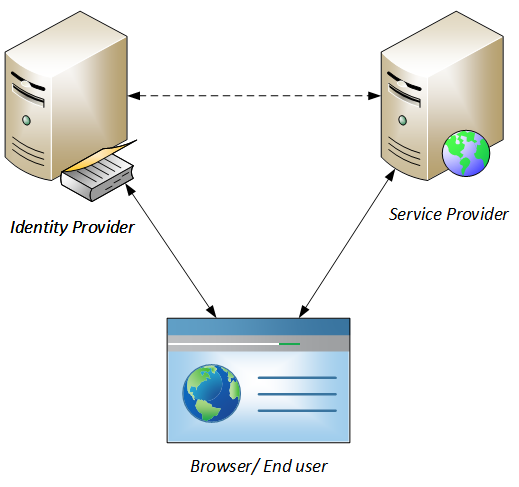
\includegraphics[scale=0.70]{graphics/Implementasjon/AutheticationFlow.png}}
    \caption{Skisse for illustrasjon av autentiseringflyt}
    \label{fig:authenticationFlow}
\end{figure}

\subsection*{SAML}
SAML\ref{sec:teoridel_SAML} omtales først og fremst som en autentisering protokoll og det er dette protokollen blir brukt til i Azure AD\cite{AadSamlSingelSignIn}. Autentiseringsflyten i protokollen er beskrevet overordnet i listen nedenfor, se figur \ref{fig:authenticationFlow}, og kan brukes for å enklere se sammenknytningen mellom sluttbruker, identity provider og applikasjon.
\\
\begin{itemize}
\item En sluttbruker (brukeren) spør en applikasjon om tilgang til beskyttede ressurser og applikasjonen håndterer ikke autentisering selv så sluttbrukeren blir sendt videre til en identity provider (Azure AD). 
\item Første gang brukeren skal logge på applikasjonen har ikke brukeren sesjonsdata som kan bevise at den er autentisert. Brukeren må derfor autentisere seg og vil bli sendt til en innloggingside. Når brukeren forsøker å logge inn på denne siden sendes forespørselen som en SAML forespørsel sammen med en "RelayState". "RelayState" er adressen brukeren skal sende tilbake dersom autentiseringen godtas. 
\item Brukerens nettleser mottar svar fra Identity Provideren ved vellykket innlogging og responsen kan sees på som en identifikasjonskode i form av en signatur. Denne signaturen lagres og videresendes til "RelayState" adressen. RelayState adressen er knyttet til applikasjonen brukeren ønsker å autentiseres for og er der brukeren må sende signaturen.
\item Applikasjonen mottar forespørselen om å åpne "RelayState" adressen sammen med SAML signaturen. Om applikasjonen godkjenner signaturen vil applikasjonen fullføre innloggingen og gi brukeren tilgang til de beskyttede ressursene.
\end{itemize}

\subsection*{OpenID Connect}
OAuth2 er mer en authorisasjonprotokoll enn en autentiseringprotokoll. OpenID Connect bygger videre på OAuth2 og fyller noen av manglene OAuth hadde. For å forklare OpenID Connect på en enkel måte må vi forklare litt rundt tokens. Mens SAML i prinsippet er basert på en etterprøvbar signatur, så baserer OpenID Connect seg på flere tokens. "Access token", "Refresh token" og "Identity token" brukes av OAuth og OpenID Connect, i tillegg benyttes en "Autentication code". I listen nedenfor blir autentiseringsflowen og bruken av tokens forklart på en forenklet måte. 

\begin{itemize}
\item En sluttbruker (brukeren) spør en applikasjon om tilgang til beskyttede ressurser. Applikasjonen håndterer ikke autentisering selv så sluttbrukeren blir sendt videre til en Identity provider (azure ad). 
\item Første gang brukeren logger på har ikke brukeren sesjonsdata lagret. Brukeren må autentisere seg og blir da sendt til en innloggingside. Etter autentiseringen mottar sluttbruker en authentiseringkode og en "redirect url". 
\item Autentiseringkoden har kort levetid. Den sendes via sluttbruker til en applikasjonsserver for å få en Access token. 
\item Applikasjonsserveren mottar forespørselen med autentiseringskoden og sender denne koden videre til Identity provideren. 
\item Identity provideren ser at tokenet er det samme som det som ble sendt til brukeren og svarer med å sende applikasjonsserveren et Access token tilbake.
\item Applikasjonsserveren sender bruker tokenet for å låse opp beskyttet data og sender både data og Access tokenet tilbake til sluttbrukeren.
\item Når brukeren skal spørre etter nye beskyttede data sender brukeren forespørsel til applikasjonsserveren med Access token.
\end{itemize}

I tillegg til Access token og autentiseringkode kan sluttbruker spørre en autentiseringsserver om to typer tokens til:
\begin{itemize}
\item Refresh token kan brukes for å få nye Access tokens uten å måtte oppgi på nytt både brukernavn og passord. Tokenet kan bli gitt av en autorisasjonserver og vil ha evig varighet. Dette betyr at så lenge brukeren ikke trekker tilbake tilgangen til en applikasjon eller logger ut så vil brukeren alltid være logget inn på applikasjonen. Refresh token kan mottas samtidig med Access tokene eller spørres etter separat.
\item Identity token er en samling av personlige data brukeren kan etterspørre fra Identity provideren. Det er designet slik at det kan etterprøves om dataene stemmer.
\end{itemize}

OpenID Connect og OAuth er bassert på JWT(JSON Web Token), mens SAML er bassert på XML (Extensible Markup Language).

\subsection{Logg ut}
\label{subsec:konfigurasjon_innloggingsmekanismer_loggUt}
For at Single Sign Out skal virke må Identity provideren vite om alle pågående autentiserte applikasjoner for hver bruker, samt kjenne til eller få beskjed om "LogoutURL". SAML og OAuth løser dette på nesten samme måte, med unntak av at pakkene som sendes er i ulike formater og med litt ulikt innhold. Applikasjoner som ikke er koblet til Identity provideren når utlogging pågår vil få en feilmelding nestegang brukeren tar de i bruk. Brukeren vil bli bedt om å logge inn igjen på nytt.

\begin{itemize}
\item Sluttbruker sender en forespørsel til en applikasjon om å logge ut av sin konto. Dette kan gjøres ved å klikke på en logg ut knapp.
\item Applikasjonen sender en "LogoutRequest", en utloggingsforespørsel, til Identitiy provideren via sluttbruker. 
\item Identity provideren logger ut brukeren og sender en "broadcast" melding til alle applikasjoner tilknyttet den autentiserte sesjonen og som identity provideren er tilknyttet.
\item Identity provideren sender en "LogoutRespons" tilbake til applikasjonen via sluttbruker og denne responsen inneholder en logg ut url. 
\item Applikasjonen ser responsen fra Identity provideren og fullfører utloggingen.
\end{itemize}

\subsection{Glemt passord}
\label{subsec:konfigurasjon_innloggingsmekanismer_glemtPassord}
Om en bruker har glemt passordet sitt til NorkartID kan brukeren trykke på lenken "Får du ikke tilgang til kontoen?" som ligger på innloggingsiden. Dette gjelder innloggingsiden levert av AAD, og brukes hver gang en bruker skal logge på en applikasjon enten det er en webapplikasjon (se implementasjonsbeskrivelse \ref{subsec:konfigurasjon_handteringAvApplikasjoner_leggTilApplikasjonIAzureAD}) eller en Android applikasjon ( se implementasjonsbeskrivelse \ref{subsec:konfigurasjon_handteringAvApplikasjoner_leggetilNyApplikasjon_androidApplikasjon}). Når denne linken blir trykket på vil brukeren bli sendt til AAD sin side for tilbakestilling av passord. Her vises en CAPTCHA test som bruker må fylle inn for å bevise at brukeren ikke er en robot. Når CAPTCHA testen er bestått, blir brukeren bedt om å velge hvilken autentiseringsmetode brukeren ønsker bruke å resette passordet. Disse alternativene må brukeren selv ha forhåndsdefinert ved et tidligere tidspunkt (se \ref{subsec:konfigurasjon_genrellHaandteringAvAad_tilbakestillingAvPassord} for konfigurasjonsbeskrivelser). Alternativene brukeren konfigurere er enten å svare på sikkerhetsspørsmål eller velge å motta en bekreftelseskode på ekstern e-post, sms eller via telefonsamtale. Under konfigurasjon kan bruker velge å registrere alle alternativene som mulige autentiseringsmekanismer eller bare en. Etter at den ekstra autentiseringsmekanismen er valgt og godkjent kan det skrives inn et nytt passord. Dette nye passordet kan deretter brukes for å logge inn på den ønskede nettsiden.\\
\\
Alle brukere må ha registrert autentiseringsdata for å bruke glemt passord funksjonaliteten. Dette kan gjøres på flere måter, enten via en registreringsportal, levert av Microsoft, eller ved pålogging på MyApps. Om ekstra autentiseringsmekanismer ikke er registrert vil MyApps spørre brukeren om å registrere dette. Registreringsportalen nås enten ved å gå direkte til \url{http://aka.ms/ssprsetup} eller via brukerportalen. Brukere kan logge seg inn i brukerportalen og trykke på "Registrer for tilbakestilling av passord". Begge metodene fungerer også om man har registrert bare noen av autentiseringsmetodene og ønsker å legge til fler, eller oppdatere eksisterende autentiseringsmetoder.
\\
\\
I registreringsportalen vil brukeren få valget om å registrere en ekstern e-post adresse, telefonnummer eller svare på sikkerhetsspørsmål. Dette avhenger av hvilke autentiseringsmetoder som er konfigurert i AAD av administratorene på forhånd. Ved registrering av ekstern e-post adresse vil brukeren motta en e-post med en verifiseringskode. Ved registrering av telefon gis valget mellom å få verifiseringskode på sms eller via telefonsamtale. Hvis sikkerhetsspørsmål er satt som autentiseringsmetode i AAD må det svares på et gitt antall sikkerhetsspørsmål.

\section{Egenadministrasjon}
\label{sec:konfigurasjon_egenadministrasjon}
Via myapps, den ferdig utviklede egenadministrasjon løsningen fra Microsoft kan man kun endre på grupperelasjoner og kjøre eventuelle applikasjoner man har tilgang til. For å kunne endre det som er nevnt i kravspesifikasjonen må det tas i bruk en egen løsning hvor man tar i bruk Windows PowerShell eller Graph API. Ved hjelp av disse tjenestene kan man gjøre det som er beskrevet i \ref{subsec:kravspesifikasjon_funksjonelleKrav_hoyNivaa}. Ved å implementere en egen brukerprofil nettside vil man kunne endre på e-post adressen, passord, mobil nummer og en rekke andre. Dette gjøres ved å bruke enten PowerShell eller Graph API og har sine restriksjoner med hva du kan endre på. Dette kan man ikke endre på men man kan endre på alle felter som er mulig å endre inne i selve Azure portalen. Passord resett kan gjøres ved å bruke myapps eventuelt ved å implementere det eksempelvis i en nettside eller applikasjon. Lager man en egen nettside klarer man å møte alle de sikkerhetskravene som er nevnt i kravspesifikasjonen.

\subsection{Endre brukerdata}
\label{subsec:konfigurasjon_egenadministrasjon_endreBrukerdata}
For å endre på brukerdata må dette gjøres utelukkende igjennom enten Graph API eller PowerShell. Hvis man logger inn på myapps for å se over sin konto samt sine tilganger til applikasjoner får man kun en oversikt over hva som er registrert på sin konto. For å endre dette må dette gjøres igjennom å lage en egen nettside eller applikasjon som endrer på disse dataene igjennom nevnte tjenester og API'er.

\subsection{Endre passord}
\label{subsec:konfigurasjon_egenadministrasjon_endrePassord}
Sluttbruker skal ha mulighet til å endre sitt eget passord. Dette er for å lette arbeidsmengden ytterligere hos kundeservice. For å gjøre dette trengs det å ha Azure Premium eller Basic, se lisensiering \ref{subsec:konfigurasjon_genrellHaandteringAvAad_lisensmodell}. Sluttbrukere kan endre sitt passord via brukeradministrasjonssiden myapps. Ved å trykke på "endre passord" i myapps må først gammelt passord oppgis. Deretter må nytt passord tastes inn to ganger og AAD har en rekke sikkerhetskrav til det nye passordet. {\color{blue} Bør vi skrive hvilke?}

\section{Brukeradministrasjon}
\label{sec:konfigurasjon_brukeradministrasjon}
Myapps fra Azure kan håndtere passord og forespørsler om grupper. Man kan gi gruppeansvar til en bruker i en gruppe og kan dermed håndtere hvilke entiteter som kan være med. Dette kan være andre brukere som forespør om de kan være med i gruppe. Myapps har ikke mulighet for å endre på informasjon knyttet til brukerne. Administreringen av flere brukere i en gruppe og kunne se samt endre på informasjon i henhold til kravspesifikasjon, beskrevet under \ref{subsec:kravspesifikasjon_funksjonelleKrav_hoyNivaa}, er mulig å oppnå ved bruk av Graph API eller PowerShell. Dette kan settes opp som en egen nettside vedsiden av Azure, eventuelt i Azure. Det kan også legges inn i applikasjoner, eksempelvis skrevet i C\#, som kan utvikles for å gjøre de ulike oppgavene som er ønsket mot brukerne. Legg til og fjerne brukere blir også håndtert av PowerShell eller Graph API. 

\section{Håndtering av brukere, roller og grupper}
\label{sec:konfigurasjon_handteringAvRollerOgGrupper}
I dette delkapitlet skal vi ta for oss ulike vurderinger og hvordan man skal gå fram for å få brukere og grupper inn i Azure.

\subsection{Masse-registrering av brukere}
\label{subsec:konfigurasjon_handteringAvRollerOgGrupper_masseRegistrering}
For å gjennomføre en masse-registrering av brukere er det flere alternativer som kan brukes for oppnå dette. Mulighetene man har er:
\begin{itemize}
\item Azure AD Sync
\item Graph API
\item PowerShell
\end{itemize}

Azure AD Sync på lokale AD'er er brukt for å synkronisere inn brukere fra lokale AD'er. Den muliggjør også å synkronisere inn multi-forests\footnote{En forest er en singel instanse av Active Directory. Multi-forests er en rekke Active Directories.} inn til AAD. Den kjører en stor initiell synkronisering hvor det sendes hele kontoer fra den lokale AD'en inn til Azure AD. Etter dette kjøres det et 3 timers intervall for å sjekke at alt er synkronisert. Dette kan endres til hvilket som helst intervall man ønsker. I tillegg til det kan man velge hvilke kontoer som skal synkroniseres ut i fra hvilken OU\footnote{OU, Organizational units, er AD sin beholder hvor man kan plassere brukere, grupper, datamaskiner og andre tjenester i organisasjonen og kan ikke inneholde objekter fra andre AD'er. Typisk brukt for å skille på brukere med samme navn} de ligger i. Ved å bruke Azure AD Sync kan du også sette på valgfrie funksjoner som  Eksempelvis "password writeback" for å synke passord tilbake til en lokal AD. Dette forsikrer deg om at endringer i passord blir skrevet tilbake til lokal AD og dermed kan dette brukes for å endre, eventuelt resette passord, gjennom Azure sine tjenester. Et resultat av dette er at brukere kan få tilgang til lokale datamaskiner som er administrert av en lokal AD ved å gå gjennom Azure tjenestene på Internett. Disse tjenestene er tilgjengelig hvor enn man er. \\
\\
Når du synkroniserer fra en eksisterende AD vil man kunne se dette på oversikten over brukere. Det vil stå "cloud" på de brukerne som ikke er i en lokal AD og det vil stå "Synced with Active Directory" for de som er både i skyen og i den lokale AD'en. De som ligger begge steder må først slettes i den lokale AD'en, for så å vente på at replikering kjøres mellom lokal AD og Azure AD, før de slettes i skyen. Man kan også importere brukere fra SQL databaser inn i Azure SQL. Ønsker man å få disse over i AAD må man gjøre dette gjennom PowerShell\footnote{Windows PowerShell er et rammeverk for konfigurasjonshåndtering og oppgave automatisering fra Microsoft som består av en kommandolinje basert skallprogram og har et skripte språk som er basert på .NET Framework.}. \\
\\
SQL databaser gjøres primært gjennom PowerShell skripting da formatet på dataen man henter ut varierer. Ved å bruke PowerShell kan man håndtere importen slik man ønsker og man har kontroll over hele prosessen. I kombinasjon med PowerShell kan man gjøre en masse registrering ved å bruke en liste av eposter hvor man ber hver og en om å gå inn for å registrere seg inn i systemet selv.

\subsection{Enkelt-registrering av brukere}
\label{subsec:konfigurasjon_handteringAvRollerOgGrupper_enkeltRegistrering}
{\color{blue} Skrive om at man kan registrere brukere direkte i Azure portalen også?}\\
For å registrere brukere kan man bruke Graph API for å lage en registreringside der man knytter seg til en Azure AD. Her kan man spørre om det man måtte trenge av detaljer og sende dette inn til AAD ved hjelp av Graph API. Ved siden av dette kan man registrere seg igjennom Azure portalen direkte også. Dette kan deretter bli knyttet til de grupper og roller man måtte ha i sin organisasjon.

\subsection{Håndtering av brukere}
\label{subsec::konfigurasjon_handteringAvRollerOgGrupper_haandteringAvBrukere}
{\color{blue} Skjønte ikke denne helt}\\
Et hendelsesforløp for brukere ville vært at når de registreres i AAD får de tildelt et midlertidig passord. Dette passordet kan man tvinge at skal endres ved første gangs innlogging. Dette medfører at brukeren blir kjent litt med hva som skjer i prosessen og kommer inn i Azure på mer eller mindre egne premisser. Siden myapps siden kommer til å være i Azure, eller om Norkart lager den selv, så er det viktig å kjenne til hvor man må gå for å nå NorkartID. NorkartID kan være en samle side for nyregistreringer, tilgang til brukerprofil og se eventuelt se tilstand i systemet med tanke på oppetid.

\subsection{Registrering av grupper}
\label{subsec::konfigurasjon_handteringAvRollerOgGrupper_grupper}
{\color{blue}Slå sammen registrering og håndtering av grupper?}\\
Ved hjelp av portalen kan man opprette de grupper man ønsker og legge inn medlemmene man vil ha i de respektive gruppene. Man har tilgang til det man måtte trenge for å opprette grupper og legge grupper inn i andre grupper. 
Powershell kan også nyttes for å opprette og håndtere grupper. 

\subsection{Håndtering av grupper}
\label{subsec::konfigurasjon_handteringAvRollerOgGrupper_grupper}
En gruppe i Azure er en samling av brukere og grupper som kan håndteres som en singel enhet. Brukere og grupper som tilhører en spesifikk gruppe vil bli omtalt som et gruppemedlem. Ved bruk av grupper kan man forenkle administreringen ved å tildele et standard sett med rettigheter og tilganger til en spesifikk gruppe. En bruker kan dermed legges inn i denne gruppen og få tilgangene og rettighetene til gruppen. I skrivende stund kan du kun lage sikkerhetsgrupper i Azure. Dette brukes for å tildele brukere tilgang til applikasjoner på gruppenivå. Ved å legge tilgang til en applikasjon mot en gruppe gjør dette det mulig å legge brukere inn i gruppen etterpå. Dette gjelder også når du håndterer tilganger til andre online tjenester. Handlinger du kan gjøre angående grupper i AAD:

\begin{itemize}
\item Lag en gruppe
\item Legg til et medlem i en gruppe
\item Fjerne et medlem i en gruppe
\item Endre en gruppes egenskaper
\item Slette en gruppe
\item Redigere gruppe eiere
\item Se rapport for gruppe aktivitet
\item Selvadministrer gruppe håndtering for brukere
\item Tildele tilgang for en gruppe til en SaaS applikasjon
\item Opprette dedikerte grupper
\item Opprette dynamisk medlemskap for grupper
\end{itemize}

\subsection*{Dynamiske Grupper}
AAD har en funksjonalitet de kaller dynamiske grupper. Dette er grupper som legger til medlemmer automatisk basert på hvilke attributter, som land eller avdeling, brukeren registrerer. Dette fører til at man da ikke går inn spesifikt for å legge en nyansatt utvikler i utviklergruppen fordi en merker av den nyansatte som utvikler, eller registrere hvilke avdeling, og AAD ordner tilgangen automatisk.

\subsection*{Gruppe Claims}
Gruppe claims gjør det lettere for skreddersydde applikasjoner å støtte deling grupper{\color{blue} ?} med andre brukere på tvers av en organisasjon. Denne typen applikasjon kan bruke gruppeinformasjon i AAD tokens for å gjøre det enklere for brukere å dele tilgang med andre brukere i organisasjonens AD. Dette forenkler deling og tilgangshåndtering ved å eliminere behovet for å håndtere gruppemedlemskap i flere applikasjoner. \cite{AppRoleOgClaims} \\
\\
Skisse over gruppeinndelingen hos oppdragsgiver tar vi ikke for oss i denne oppgaven, da vi antar oppdragsgiver ønsker å ta i bruk egne erfaringer med tidligere AD bruk i sin kommende AAD løsning. Oppdelingen av disse gruppene kan eksempelvis gjøres ved at man har grupper som representerer leserettigheter på en applikasjon, mens en annen grupper gir både lese og skriverettigheter på en applikasjon. Azure løser dette i henhold til administreringskravene satt i kravspesifikasjonen \ref{subsec:kravspesifikasjon_funksjonelleKrav_hoyNivaa}.

\subsection{Håndtering av roller}
\label{subsec::konfigurasjon_handteringAvRollerOgGrupper_roller}
Roller i Azure er et sett med handlinger som kan gjøres mot en Azure ressurs. En bruker kan utføre en handling på en Azure ressurs hvis de har blitt tildelt en rolle som inneholder denne handlingen. Azure har en rekke innebygde roller hvor hver av dem kan utføre ulike handlinger. Det er også mulighet for å opprette sine egne roller og tildele handlingene man ønsker. En rolle kan også tildeles til en tjeneste og vil kunne utføre det samme som en bruker. Roller kan du tildele til brukere, grupper eller tjenester. De rollene som Norkart trenger for å møte kravspesifikasjonen er \\
\begin{itemize}
\item Super administrator
\item Kundestøtte bruker
\item Lokal administrator
\item Sluttbruker
\end{itemize}
I Azure er det disse alternativene for brukere
\begin{itemize}
\item Billing administrator håndterer kjøpene, avtaler, tjenesteforespørsler  og overvåker tilstanden til tjenester.
\item Global administrator har tilgang til alle administrative tjenester og det kan kun være en i en organisasjon. Dette er den som skriver seg opp som Azure kontoholder. Det er kun denne rolle som kan tildele andre brukere administrator roller.
\item Password administrator resette passord, håndtere tjeneste forespørsler, og overvåker tjeneste tilstand. Man kan også resette passord bare for brukere og andre password administrators.
\item Service administrator håndtere tjenesteforespørsler og overvåker tilstanden til tjenstene.
\item User administrator resette passord, overvåker tjeneste tilstand og håndterer bruker kontoer, bruker grupper og tjeneste forespørsler. Det er noen begrensninger her, for eksempel kan kan ikke disse slette global administratoren eller lage andre administratorer. I tillegg kan de ikke resette passord for billing, global eller service administratorer.
\end{itemize}

Super administrator vil her være Service administrator. Kundestøtte bruker er User administrator og Lokal administrator er User administrator. Slutt bruker ville vært en user da det ikke er behov for administrator rettigheter på ordinære sluttbrukere.

\subsection*{Applikasjons rolle}
Dette muliggjør for utviklere til å deklarere et sett med roller i Azure AD som en applikasjon trenger for å autentisere. Brukere får tildelt roller og i innloggingøyeblikket avgjøre Azure AD hvilken rolle en bruker har og inkluderer dette i tokenet. Applikasjoner kan inspisere dette tokenet og bruke rollen som står for å autentisere bruker. Dette kan brukes for å si hvem som har tilgang til hvilken applikasjon og dette kommer til å være lagret på en sentral lokasjon, i Azure AD. \cite{AppRoleOgClaims}

\section{Håndtering av applikasjoner}
\label{sec:konfigurasjon_handteringAvApplikasjoner}
Denne seksjonen forklarer hva Norkart må ta hensyn til angående applikasjoner som skal benytte seg av AAD som en autentisering- og  autoriseringløsning. Applikasjonene må være registrert i en AAD og kan registreres og konfigureres i Azure portalen. I tillegg må det implementeres litt logikk i applikasjonene.

\subsection{Registrere applikasjon}
\label{subsec:konfigurasjon_handteringAvApplikasjoner_leggTilApplikasjonIAzureAD}
For at AAD skal klare å kommunisere med applikasjonene og vite hvilke rettigheter de har så trengs det en del informasjon. Hva slags informasjon og hvorfor den trengs \cite{RegistrereApplikasjoneriAAD} står beskrevet her:
\bigskip
\begin{description}
    \item [Applikasjons URI] \hfill \\ 
    Applikasjons URI er identifikatoren til en applikasjon. URI'en blir brukt når en bruker skal autentiseres for applikasjonen. Den blir sendt til AAD og forteller at det er denne applikasjonen brukeren ønsker token til. URI'en er i tillegg inkludert i tokenet, slik at applikasjonen vet at det var til seg brukeren ville. 
    \bigskip
    \item [Reply URL og redirect URL] \hfill \\
    Dette er URL'er AAD sender autentiseringrespons og token til, dersom autentisering lykkes. 
    \bigskip
    \item[Klient id og nøkkel] \hfill \\
    Klient id blir generert av AAD når applikasjonen registreres og er applikasjonens id. Denne brukes sammen med en nøkkel(client secret) når applikasjonen trenger tilgang til AAD gjennom Graph API eller andre API'er. Applikasjonen bruker nøkkelen og klient id for å be om Access token fra AAD OAuth 2.0 token endpoint. Token endpoint bruker da klient id og nøkkel til å autentisere applikasjonen før den sender ut et Access token.
\end{description} 
\bigskip

Applikasjoner i en AAD kan være kategorisert som enten single tenant eller multi tenant. Dette vil si om applikasjonene skal kunne kobles til flere AAD eller om alle brukerene av applikasjonen må ligge i samme AAD for hver enkelt installasjon av applikasjonen. Multi-tenant applikasjoner er som regel SaaS funksjoner. Nærmere forklaring om single tenant og multi tenant applikasjoner kan finnes i teori kapittelet under \ref{sec:singleTenantApplikasjon} og \ref{sec:multiTenantApplikajson}. For veiledning til hvordan applikasjoner kan registreres i en AAD, se brukerveiledning for dette i seksjon \ref{subsec:veiledninger_brukerveiledningForWebApplikasjon_registreringAvWebApplikasjoneriAad}, i kapittelet \ref{chap:veiledninger} \refname{chap:veiledninger}. Veiledningene viser registrering av single tenant applikasjoner. Konfigurering av multi-tenant applikasjoner blir ikke diskutert i denne oppgaven ettersom oppdragsgiver ikke har behov for dette. \ref{subsec:konfigurasjon_handteringAvApplikasjoner_konfigurereApplikasjonIAzureAD} \\

\subsection{Konfigurere applikasjon}
\label{subsec:konfigurasjon_handteringAvApplikasjoner_konfigurereApplikasjonIAzureAD}
Applikasjoner som er registrert i en AAD kan konfigureres i Azure portalen. Her kan applikasjonens tilgang til andre applikasjoner og web API'er settes, applikasjonsdata som URL, APP ID URI og logo kan endres samt brukerens adgang kan bestemmes. Denne seksjonen forklarer hvordan en single-tenant applikasjon kan gjøres om til å være multi-tenant, hvordan eksponere et web API, hvordan applikasjonen får tilgang til Graph API og hvilke regler som kan settes for brukeradgang til applikasjonen. Denne seksjonen er basert på Microsoft sine forklaringer rundt håndtering av applikasjoner i en AAD. \cite{AddingUpdatingRemovingApplications}

\subsection*{Konfigurere multi-tenant applikasjoner}
For å gjøre en single-tenant applikasjon om til en multi-tenant applikasjon må dette aktiveres under applikasjonens konfigurasjonsfane. Sett "Application is multi-tenant" til yes og lagre. Mulit-tenant applikasjoner må ligge både i bedriftens AAD og i alle AAD som har brukere som skal benytte seg av applikasjonen. Brukerne vil da få se hvilke rettigheter applikasjonen har og godkjenne disse. Når dette gjøres for native applikasjoner er det kun web API'et som ligger i brukernes AAD. 

\subsection*{Web API}
Hvis oppdragsgiver ønsker å eksponere et web API til andre applikasjoner i AAD kan dette gjøres ved å laste ned manifestet til API'et og endre OAuth 2.0 rettighetene. Manifestet kan lastes ned ved å trykke på "Manage manifest" i bunnmenyen. Bytt ut innholdet i JSON manifestet til:

\begin{lstlisting}[caption={JSON manifest},label={lst:JSON_manifest}]
   "oauth2Permissions": [
    {
      "adminConsentDescription": "Allow the application full access to the Todo List service on behalf of the signed-in user",
      "adminConsentDisplayName": "Have full access to the Todo List service",
      "id": "b69ee3c9-c40d-4f2a-ac80-961cd1534e40",
      "isEnabled": true,
      "origin": "Application"
      "type": "User",
      "userConsentDescription": "Allow the application full access to the todo 
      service on your behalf",
      "userConsentDisplayName": "Have full access to the todo service",
      "value": "user_impersonation"
    }
  ],
\end{lstlisting}

Bytt ut teksten til å passe API'et. Id'en er en unik identifikator for rettighetene som gis av API'et og denne må være en GUID. Last så opp det nye manifestet i Azure portalen. Web API'et vil nå være tilgjengelig for andre applikasjoner.

\subsection*{Få tilgang til Graph API}
Hvis applikasjoner trenger tilgang til Graph API kan dette konfigureres under "permissions to other applications". Tilgang til Graph API, er satt som standardinnstilling for alle applikasjoner i AAD og kalles Windows Azure Active Directory. Tilgangen applikasjonen trenger fra Graph API, som lese og skrive rettigheter eller kun lese rettigheter kan også settes her. 

\subsection*{Adgangsregler}
I AAD er det mulig å sette en del adgangsregler for hvilke brukere som skal ha adgang til applikasjonen og hvordan. Denne funksjonaliteten er i skrivende stund kun tilgjengelig som preview. Adgangsreglene for en applikasjon kan gjelde for alle brukere, spesifikke brukere eller spesifikke grupper. Så langt i Azure sitt livsløp er det kun mulig å sette regler for multifaktor autentisering. Det kan konfigureres om multifaktor autentisering alltid skal brukes eller at det kun skal brukes dersom brukere logger seg inn via usikre nettverk. Dette gjøres ved å sette hvilke nettverk som er trygge i Azure Portalen. Det er også mulig å la brukere utsette multifaktor autentisering ved å huske sine enheter i 1 - 60 dager. \\
\\
I følge Alex Simons, direktør for programledelse i Microsofts identitets og sikkerhetsdivisjon, vil det bli mulig å sette flere typer adgangsregler i fremtiden\cite{AccessRules}. Microsoft forklarer at det vil komme flere typer adgangsregler som kan settes i fremtiden, men sier ikke når.

\subsection{Implementering av Webapplikasjon - ASP.NET MVC}
\label{subsec:konfigurasjon_handteringAvApplikasjoner_Webapplikasjon}
Applikasjoner som skal bruke AAD som autentiseringsverktøy må implementere en del elementer. For webapplikasjoner må det blant annet legges inn noen biblioteker for å kunne benytte OIDC protokollen og litt informasjon som AAD trenger for å autentisere brukere opp mot applikasjonen. \\
\\
For at applikasjonen skal bruke AAD autentisering via OIDC protokollen må den være en OWIN basert applikasjon. Dette gjøres ved å installere Katana elementene OWIN system.web og OWIN security. Se \ref{lst:katana_elementer} OWIN security pakken gjør det mulig å velge OIDC som autentiseringsprotokoll. \cite{WebappTutorialCloudIdentity}

\begin{lstlisting}[caption={Katana elementer},label={lst:katana_elementer},numbers=left,escapeinside={@}{@}]
Install-Package Microsoft.Owin.Security.OpenIdConnect -Pre
Install-Package Microsoft.Owin.Security.Cookies -Pre
Install-Package Microsoft.Owin.Host.SystemWeb -Pre
\end{lstlisting}

\bigskip
I tillegg til Katana elementene må det implementeres litt logikk i applikasjonen. Det må lages klasser for å konfigurere autentisering og disse kommer til å bruke Owin mellomvaren og setter OIDC som autentiseringsprotokoll. I tillegg kan det her settes mange egenskaper for OIDC. For at OIDC protokollen skal fungere er det kun nødvendig å sette noen få egenskaper, se \ref{lst:satrtup_auth_cs}. Egenskapene som trengs er applikasjonens id i AAD (klient id), metadata som trengs for å motta nøkler fra AAD, altså innloggingsurl til AAD tenanten. URL som bruker skal sendes til, etter logg ut, kan også settes her. 

\begin{lstlisting}[caption={Startup.Auth.cs},label={lst:satrtup_auth_cs},numbers=left,escapeinside={@}{@}]
app.UseOpenIdConnectAuthentication(
    new OpenIdConnectAuthenticationOptions
    {
        ClientId = clientId,
        Authority = authority,
        PostLogoutRedirectUri = postLogoutRedirectUri
    });
\end{lstlisting}

\bigskip
I applikasjoner som ikke bruker innlogging fra før må det legges til et logg inn view som må refereres til i layout filen og en controller som behandler innlogging og utlogging. Slik får applikasjonen logg inn og logg ut knapper med funksjonalitet i hovedmenyen. Controlleren, se \ref{lst:account_controller_cs}, har ansvaret for å sende innloggings og utloggingsforespørsler til Owin og OIDC. 

\begin{lstlisting}[caption={AccountController.cs},label={lst:account_controller_cs}]
public class AccountController : Controller
{
    public void SignIn()
    {
        // Send an OpenID Connect sign-in request.
        if (!Request.IsAuthenticated)
        {
            HttpContext.GetOwinContext().Authentication.Challenge(
                new AuthenticationProperties { RedirectUri = "/" }, 
                OpenIdConnectAuthenticationDefaults.AuthenticationType);
        }
    }
    public void SignOut()
    {
        // Send an OpenID Connect sign-out request.
        HttpContext.GetOwinContext().Authentication.SignOut(
            OpenIdConnectAuthenticationDefaults.AuthenticationType, 
            CookieAuthenticationDefaults.AuthenticationType);
    }
}
\end{lstlisting}

\bigskip
For at AAD skal kunne autentisere brukere opp mot applikasjonen må det settes fire verdier i web.config filen under
<AppSettings>, se \ref{lst:web_config}. 

\begin{itemize}
    \item ClientId blir forklart nærmere under seksjonen Registrere applikasjoner i \ref{subsec:konfigurasjon_handteringAvApplikasjoner_Webapplikasjon}
    \item AADInstance vil si hvilken instanse av Azure som brukes. Her brukes https://login.windows.net/{0} som er den offentlige Azure AD instansen.
    \item Tenant er navnet, eller domene til den aktuelle  AAD tenanten. Dette kan være et domene gitt av Azure eller det kan være et eget domene som er registrert for den aktuelle AAD.
    \item PostLogoutRedirectUri er URL'en brukerne vil bli viderekoblet til etter utlogging
\end{itemize}

\begin{lstlisting}[caption={Web.config},label={lst:web_config}]
    <add key="ida:ClientId" value="1ef05302-c640-4459-a2b1-3c660c9854db" />
    <add key="ida:AADInstance" value="https://login.windows.net/{0}" />
    <add key="ida:Tenant" value="NorkartIDDevelopment.onmicrosoft.com" />
    <add key="ida:PostLogoutRedirectUri" value="https://norkartidman.azurewebsites.net/" />
\end{lstlisting}

\bigskip
For å sikre kommunikasjon mellom webapplikasjon og AAD er det viktig at SSL aktiveres i applikasjonen.

Kodeeksemplene presentert i denne seksjonen er i hovedsak hentet fra et kodeeksempel i GitHub under AzureAD Samples som heter WebApp-OpenIDConnect-DotNet \cite{WebAppOpenIDConnectDotNet}. Microsoft referer til dette kodeeksemplet flere steder på deres sider når det gjelder implemenetring av AAD som autentiseringsverktøy for webapplikasjoner.

\subsection{Implementering av Android-applikasjon}
\label{subsec:konfigurasjon_handteringAvApplikasjoner_leggetilNyApplikasjon_androidApplikasjon}
For å knytte Android applikasjoner til Azure for å bruke AAD som autentisering er det flere ting som må gjøres. Dette delkapitlet vil forklare overordnet hvilke elementer som må knyttes sammen og hvorfor, mens det i punkt \ref{sec:veiledninger_androidBrukerveliedning} er lagt ved en fullstendig brukerguide som viser hvordan dette kan gjøres ved bruk av en eksempelapplikasjon. \\
\\
\subsubsection{Mobile Services}
Mobile Services er en Azure tjeneste som gjør det enkelt å koble mobile applikasjoner mot en backend server med database, serverlogikk, autentisering og skalerbarhet. Vår eksempelapplikasjon tar utgangspunkt i en mobile-service backend for å teste lagring i en Azure database. Eksempelet ( se \ref{sec:veiledninger_androidBrukerveliedning}) viser litt bruk av backend logikk og programmering av ytterligere API kall. \\
\\
Norkart har applikasjoner og tjenester som bruker data fra flere større databaser. Her er det mulig å programmere applikasjoner som jobber direkte mot disse databasene, eller lage backend logikk som jobber mot eksterne databaser, for så å sende data fra eksterne databaser tilbake til brukerne igjennom azure mobile services.\\
\\
For å bruke Azure AD som autentisering for en applikasjon må man først opprette en applikasjon i Mobile Services, for deretter å knytte den til en Identity Provider. I tillegg kan det være hensiktsmessig å begrense rettighetene i databasen til kun autentiserte brukere.

\subsubsection{Azure Active Directory}
For alle typer applikasjoner som skal knyttes mot AAD må det opprettes en applikasjon i AAD. Denne applikasjonen må så knyttes mot applikasjonen opprettet i Mobile Services. Hvordan disse applikasjonene knyttes sammen gjøres ved hjelp av en applikasjons URL og en client ID, se gjerne brukerveiledningen i kapittel \ref{subsec:veiledninger_androidBrukerveliedning_del2-LeggInnAutentiseringIApplikasjonen} for en beskrivelse av hvordan dette gjøres. \\
\\
Etter det prosjektgruppen har funnet ut så må alle autorisasjonnivåer internt i en applikasjon håndteres av applikasjonens egen database og kode. Når AAD fungerer som Identity provider gir den kun tilgang eller ikke tilgang til selve applikasjonen. Men ettersom AAD støtter OpenID kan applikasjonen også få vite av AAD hvilken bruker som har fått tilgang og autorisasjon kan bygges utifra denne informasjonen. 

\subsubsection{Android kode}
Det å få en Android applikasjon til å fungerer hensiktsmessig i forhold til autentiseringsfunksjonalitet kreves det at hele applikasjonen skrives for å støtte autentisering. I eksempelapplikasjonen som bygges i brukerveiledningen i kapittel \ref{sec:veiledninger_androidBrukerveliedning} legges det inn autentisering for å åpne applikasjonen og dersom autentiseringsprosessen ikke blir vellykket avsluttes applikasjonen. Dette er ikke nødvendigvis den beste måten å implementere autentisering for alle applikasjoner. Brukerguiden viser likevel at det er få kodelinjer som skal legges til i Android for å bruke AAD som Identity provider for en applikasjon. Kodelinjene tar ibruk biblioteker som delvis bruker lokale funksjoner og delvis bruker webview mot AAD pålogging. Det er klare likheter mellom webviewet for innlogging fra en Androidapplikasjon og innlogging til en webapplikasjon fra en nettleser. Også i innloggingen i Android applikasjonen er det lagt inn branding ved hjelp av bedriftslogo og glemt-passord funksjonalitet.

\section{Generell konfigurasjon av AAD}
\label{sec:konfigurasjon_genrellHaandteringAvAad}
Konfigurasjon av Azure AD som en Identity Provider gir administrator mulighet til å endre og tilpasse på en rekke parametere. Det er blant annet mulig å konfigurere tilbakestilling av passord, generell forvaltning av grupper, applikasjons proxy og bruker adgang. Prosjektgruppen anser mye av innstillingene som kan settes som selvforklarende (se skjermbilde på figur \ref{fig:KonfigAvAzureAD}). Vi har derfor valgt og kun beskrive noen få av konfigurasjonsmulighetene nærmere.  

\begin{figure}[h]
    \centering
    \setlength{\fboxsep}{0pt}%
    \setlength{\fboxrule}{1pt}%
    \fbox{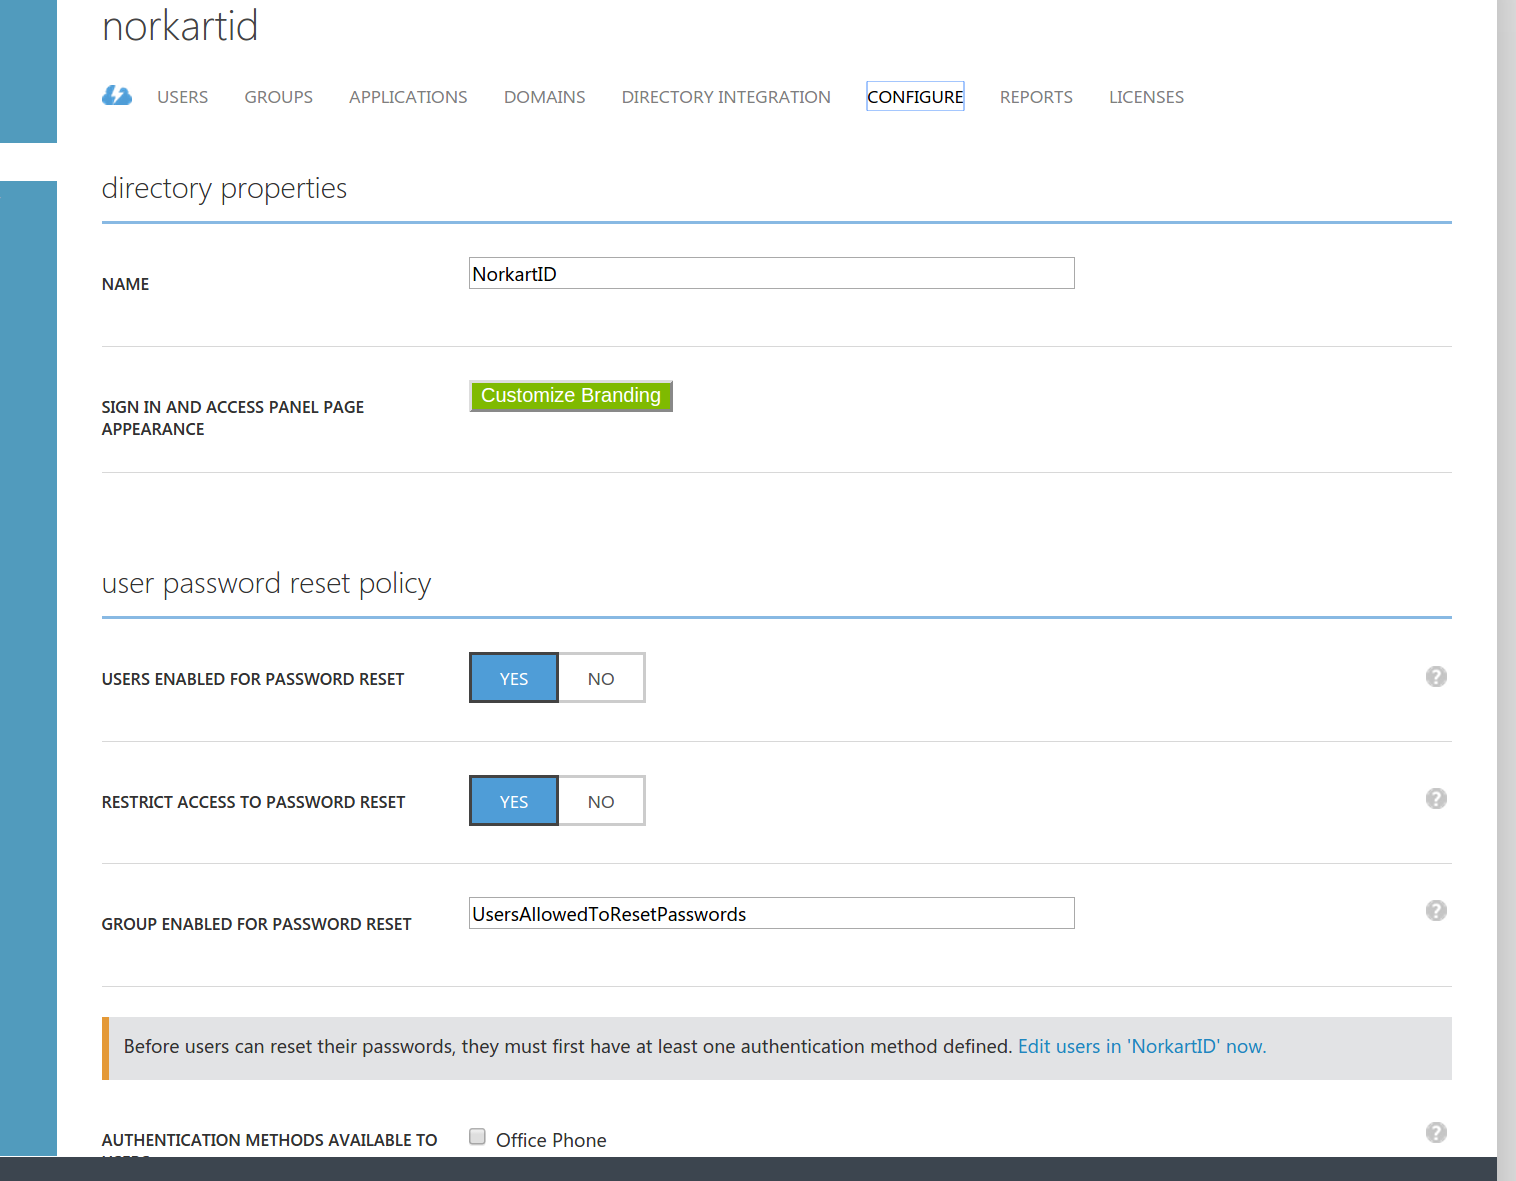
\includegraphics[scale=0.24]{graphics/Implementasjon/AzureADkonfigurasjon.png}}
    \caption{Generell overordnet konfigurasjon av Azure AD}
    \label{fig:KonfigAvAzureAD}
\end{figure}


\subsection{Lisensmodell}
\label{subsec:konfigurasjon_genrellHaandteringAvAad_lisensmodell}
Azure AD har en egen lisensieringsmodell i forhold til Azure tjenester. I skrivende stund (17 April 2015) er det ikke sluppet en offisiell B2C eller B2B tjeneste for AAD. Prosjektgruppen har vært i kontakt med Microsoft ansatte som ikke kan bekrefte eller avkrefte i forhold til hemmelighold, men som indikerer at denne funksjonaliteten vil slippes i nærmeste framtid. Om Norkart skulle basert seg på dagens lisensmodell vil brukere som knytter seg til NorkartID trolig måttet ha en Premium lisens for hver enkelt bruker. \\
\\
Lisensmodellen i Azure AD er lagt på hver enkelt bruker i brukerdatabasen \cite{AzureADPricing}. Første nivå kalles "Free" som er gratis for de første 500 000 brukerene. Andre nivå heter "basic" som det ikke finnes noen fast pris på, men må forhandles fram mellom bedriften og Mircosoft for hvert enkelt samarbeidsavtale. Siste nivået kalles "Premium" og lisensieres per bruker og koster i skrivende stund i underkant av 37 kr per bruker i måneden. Premium vil gi tilgang til det Azure AD har av funksjonalitet og tilby dette for hver eneste bruker. Muligheten til å endre passord selv, bruk av flerfaktor autentisering og mulighet for tilknytning til fler enn 10 applikasjoner per bruker er kun tilgjengelig for Premium brukere. Dette vil si at dersom Norkart har 1000 brukere de skal knytte til NorkartID igjennom Azure AD vil dette koste dem ca 37 000 kr i måneden, og ca 435 000 i året. Microsoft ønsker ikke å si noe om lisensieringsmodellene for de nye tjenestene B2C og B2B, men indikasjoner tilsier at det vil bli litt rimeligere. Prosjektgruppen har ikke lykkes med å få noen annen bekreftelse enn hva Nasos Kladakis, "Product Marketing Manager" for Azure AD, sier under en konferanse i November 2014 \cite{NasosAzureADExplained} om at begge tjenestene slippes innen et år. Da prosjektgruppen tok kontakt direkte med Kladakis kunne han hverken bekrefte eller avkrefte hva som ville slippes, men kom med indikasjoner på at det ville skje noe under Microsoft Build\cite{MicrosoftBildConference} konferansen i slutten av April 2015.

\subsubsection{Tilbakestilling av passord}
\label{subsec:konfigurasjon_genrellHaandteringAvAad_tilbakestillingAvPassord}
{\color{blue} Skal dette være med?} \\
For at brukere skal kunne egenadministrere passord for sin konto må dette aktiveres under konfigurasjonsfanen til aktuell AAD i Azure portalen. Det kan settes at det kun er brukere i en spesifikk gruppe som skal kunne gjøre dette. Hvilke autentiseringsmetoder som skal brukes og hvor mange kan også konfigureres. Det kan velges opp til to autentiseringmetoder. Valgene her er å autentiseres via jobbtelefon, mobiltelefon, ekstern e-post adresse eller sikkerhetsspørsmål. Hvis sikkerhetsspørsmål velges er det mulig å konfigurere antall spørsmål, samt eksempler på spørsmål. \\
\\
Dette vil si alle brukere som skal kunne endre sitt eget passord må registrere gjeldene autentiseringssdata. For å sikre at brukere gjør dette kan det aktiveres at bruker må registrere autentiseringsdata neste gang brukeren logger inn i brukerportalen. Antall dager før neste gang bruker må kontrollere sin autentiseringsdata kan også konfigureres her. Hvis bruker møter på problemer når passord skal endres vises en "kontakt din administrator" lenke. Denne kan konfigureres og settes til en spesifikk e-post adresse eller en URL. Hvis dette ikke settes vil det sendes en e-post til maks hundre administratorer hvor bruker spør om å få resatt sitt passord.\\
\\
Under konfigurasjonsfanen i AAD ligger det en lenke til en registreringsportal for brukere. Denne linken fungerer i skrivende stund (13.04.2015) kun for Microsoft kontoer, den vil da ikke fungere for Norkart sine AAD brukere.